\begin{frame}
\frametitle{Приоритетное планирование}

Назначим каждому потоку приоритет. Приоритет может определять:
\begin{itemize}
  \item порядок - более приоритетные идут вперед;
  \item размер кванта - более приоритетные работают дольше;
\end{itemize}

\onslide<2->{Приоритет может назначаться
\begin{itemize}
  \item статически (например, SJF - приоритет определяется длинной задачи);
  \item динамически - приоритет меняется в процессе работы (например, SCTF);
\end{itemize}}
\end{frame}

\begin{frame}
\frametitle{Shortest Completion Time First}

То же самое, что и SJF, но теперь мы можем снять задачу с процессора:
\begin{itemize}
  \item мы можем захотеть перепланировать, если появилась новая задача;
  \item приоритет - оставшееся время выполнения задачи (динамический - изменяется, когда задача выполняется);
\end{itemize}
\end{frame}

\begin{frame}
\frametitle{Старвация в SCTF}

\begin{figure}
  \only<1>{\centering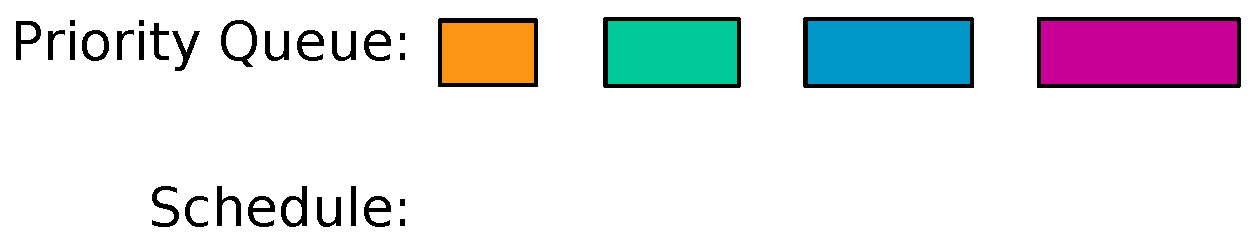
\includegraphics[width=.9\linewidth]{sctf0}}
  \only<2>{\centering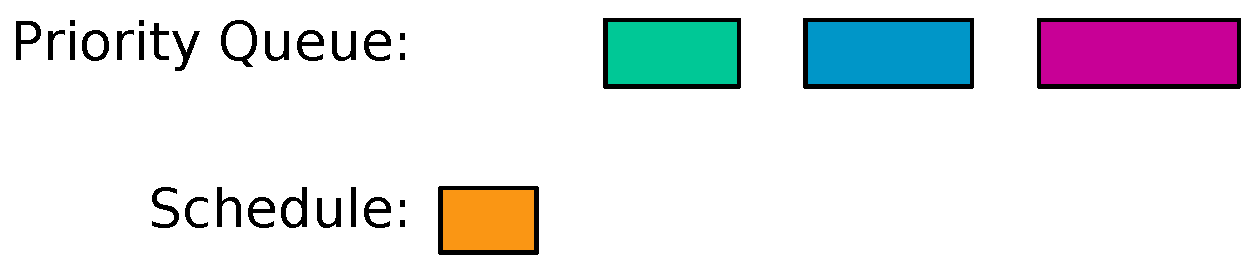
\includegraphics[width=.9\linewidth]{sctf1}}
  \only<3>{\centering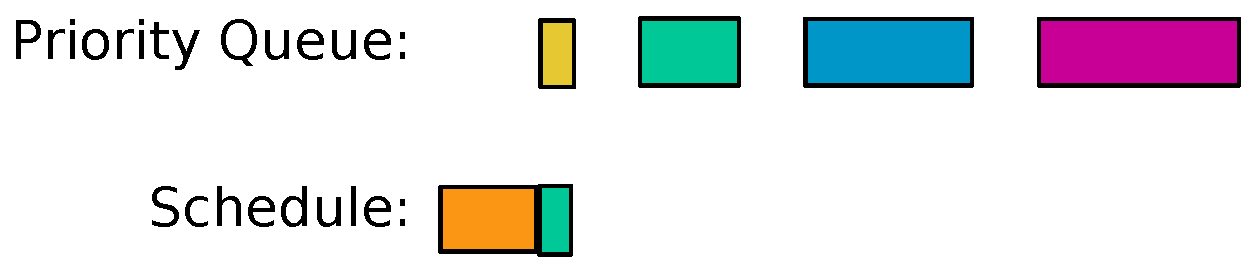
\includegraphics[width=.9\linewidth]{sctf2}}
  \only<4>{\centering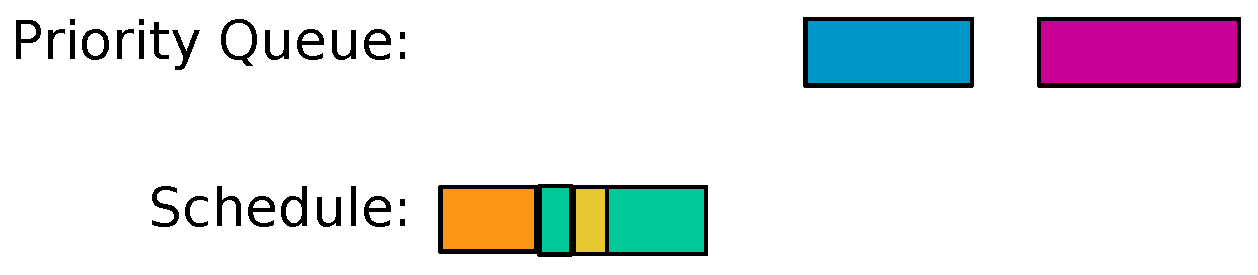
\includegraphics[width=.9\linewidth]{sctf3}}
  \only<5>{\centering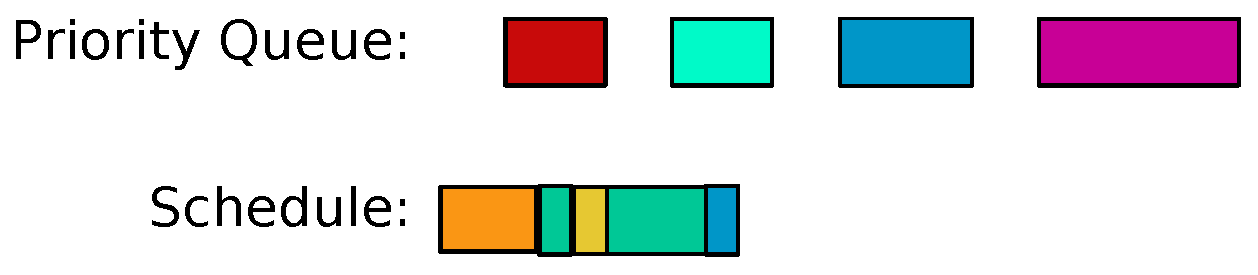
\includegraphics[width=.9\linewidth]{sctf4}}
  \only<6>{\centering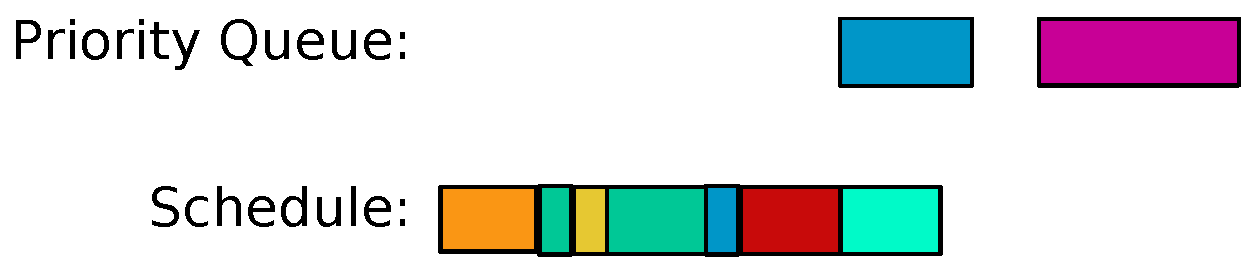
\includegraphics[width=.9\linewidth]{sctf5}}
  \only<7>{\centering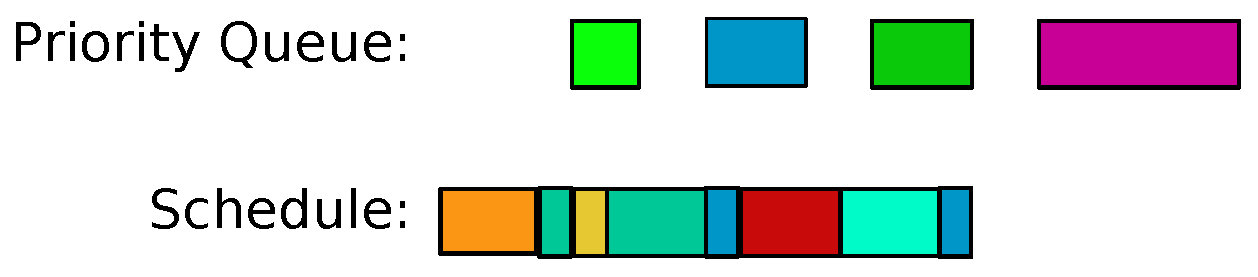
\includegraphics[width=.9\linewidth]{sctf6}}
  \only<8>{\centering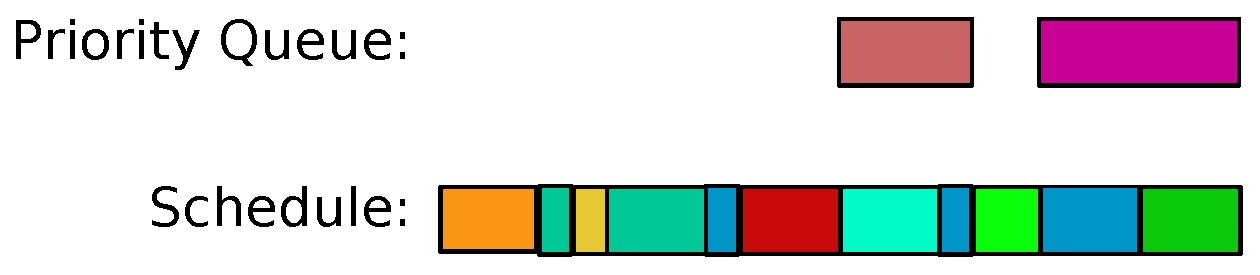
\includegraphics[width=.9\linewidth]{sctf7}}
  \caption{SCTF Example}
\end{figure}
\end{frame}

\begin{frame}
\frametitle{Multi Level Feedback Queue}

Заведем несколько очередей (по очереди на приоритет):
\begin{itemize}
  \item<1-> исполняем потоки из самой приоритетной очереди;
  \item<2-> очередь потока меняется в завивисмости от "истории":
        \begin{itemize}
          \item выработал свой квант - понижаем приоритет и увеличиваем квант;
          \item не выработал свой квант - повышаем приоритет и уменьшаем квант;
        \end{itemize}
  \item<3-> все потоки начинают с наибольшим приоритетом и наименьшим квантом;
        \begin{itemize}
          \item в оригинальной версии очередь определялась размером программы;
          \item Fernando J. Corbató получил премию Тьюринга (не только за это);
        \end{itemize}
\end{itemize}
\end{frame}
